
%%%
%%% CHAPTER
%%%
\chapter{Second Law of Thermodynamics}\label{Chapter:FirstLaw}

   \begin{LearningObjectivesBlock}{Learning Objectives}
      Upon completion of this chapter, you will be able to
        \begin{enumerate}
           \item Demonstrate understanding of key concepts of energy and the first law of thermodynamics;
           \item Apply the first law of thermodynamics to assess of heat transfer and power cycles;
           \item Conduct energy analysis of thermodynamic systems;
           \item Employ energy and mass balances into thermodynamic systems to assess efficiency, and correctly observe sign conventions for work and heat transfer.
        \end{enumerate}
\medskip
     Recommended reading: Chapters 5 of \citet{SmithVanNess_Book,Moran_Book,Borgnakke_Book} or 3 of \citet{Atkins_Book}.
   \end{LearningObjectivesBlock}


  
%%%
%%% SECTION
%%%
   \section{Introduction}\label{Chapter:SecondLaw:Section:Intro}
   The first law (Chapters~\ref{Chapter:Introduction} and \ref{Chapter:FirstLaw}) demonstrated that energy can flow either from or to a system in the form of heat or work, however it does not indicate the direction of process (\ie energy flow). The second law of thermodynamics concerns about feasibility, direction and spontaneity of processes and entropy..
   
The second law of thermodynamics is a general principle which makes constraints upon spontaneity of the process, direction of heat transfer and general efficiency of heat engines, \eg a hot body cools to the temperature of the surroundings or a chemical reaction that may run in one direction instead of the reverse (\eg combustion of ethane producing carbon dioxide and water). The reverse of such processes may occur but they will not be spontaneous.  
  
%%%
%%% SECTION
%%%
   \section{Statement of the Second Law}\label{Chapter:SecondLaw:Section:SecondLawStatement}\index{Laws of Thermodynamics ! Second law}
The second law of thermodynamics was stated separately by \citet{Clausius_Book}, Kelvin \citep{Thomson_1851} and \citet{Planck_Book} in slightly different ways. Each statement is based on irreversible processes.
\begin{shaded}
  \begin{center}
    {\bf Clausius Statement}
  \end{center}
  'It is impossible for a self-acting machine working in a cyclic process unaided by any external agency, to convey heat from a body at a lower temperature to a body at a higher temperature.'
\end{shaded}
This statement clearly indicates that heat cannot spontaneously flow from a colder to a hotter body. This can only be realised if other effects play some role, \eg in a refrigeration process in which external work is used to extract heat from low temperature body and reject it into a high temperature body.

\begin{shaded}
  \begin{center}
    {\bf Kelvin-Planck Statement}
  \end{center}
  'It is impossible to construct an engine, which while operating in a cycle produces no other effect except to extract heat from a single reservoir and do equivalent amount of work.'
\end{shaded}
This statement indicates that in order to achieve net work from a heat engine (\ie a device operating in cycle), there should be heat interaction between two bodies (\ie thermal reservoirs) at different temperatures (\ie thermal source or sink).


   %%% FIGURE
   \begin{figure}[h]
    \begin{center}
     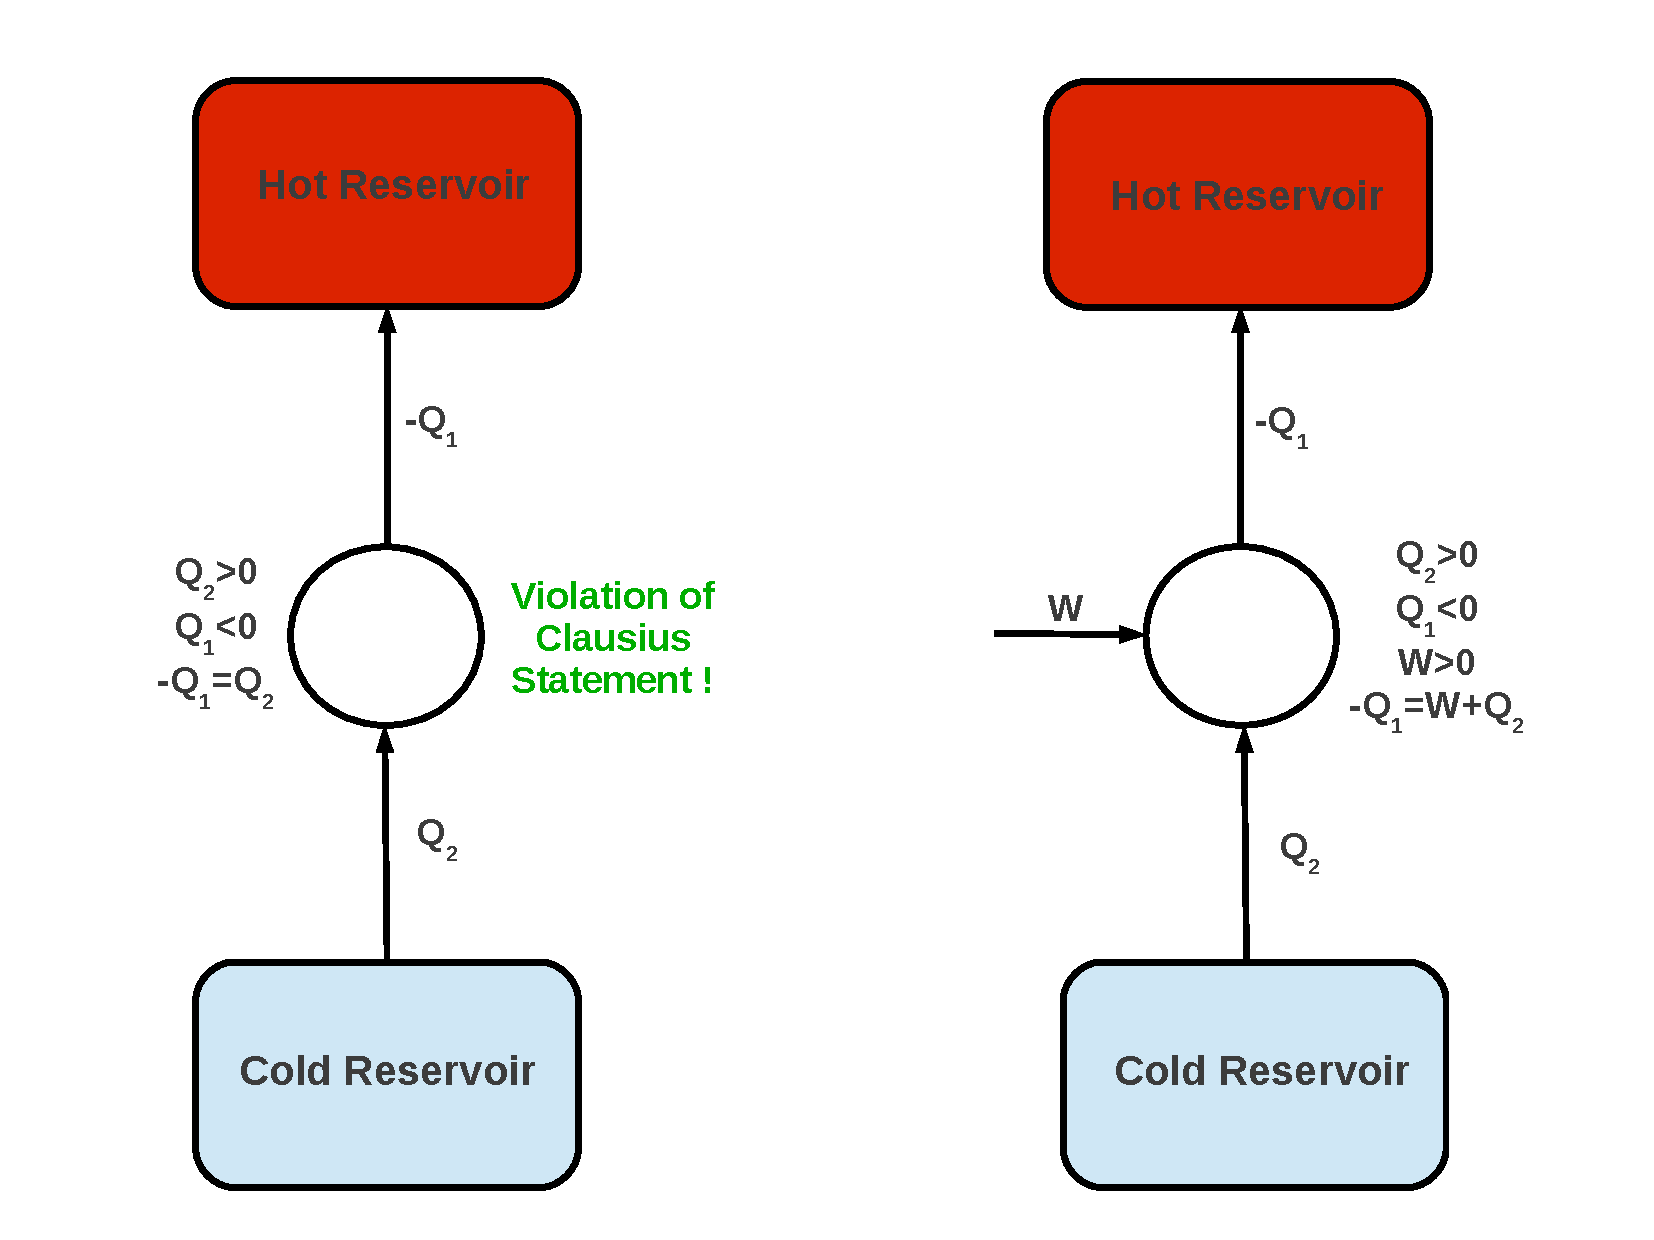
\includegraphics[width=.6\columnwidth,clip]{./Figs/2ndLaw_Schem}
     \vspace{-.1cm}\caption{All spontaneous processes are irreversible -- heat flows from hot to cold spontaneously and irreversibly.}\label{Chapter:SecondLaw:Fig:SecondLawStatement}
    \end{center}
   \end{figure} 
